\documentclass[10pt]{article}
\usepackage[margin=0.8in]{geometry}
\usepackage{mathtools,amssymb,bm,booktabs,graphicx}
\usepackage[T1]{fontenc}
\usepackage{mathptmx}
\usepackage{enumitem}
\setlist{nosep,leftmargin=1.4em}
\setlength{\parskip}{4pt}\setlength{\parindent}{0pt}
\pagestyle{plain}
\newcommand{\logit}{\operatorname{logit}}
\newcommand{\N}{\mathcal{N}}
\newcommand{\C}{\mathrm{C}}
\newcommand{\U}{\mathrm{U}}
\begin{document}
\begin{center}\textbf{A global model of where unrest leads to conflict: model equations}\end{center}

\section*{Notation}
\begin{tabular}{@{}ll@{}}
$s$, $t$ & $0.5^\circ$ cell, week \\
$j \in \{\C, \U\}$ & outcome: conflict, unrest \\
$c(s)$, $r(s)$ & country and region of cell $s$ (Africa, Middle East, South and Southeast Asia, Latin America) \\
$y(t)$ & calendar year of week $t$ \\
$g(s)$, $k(t)$ & coarse cell ($1^\circ$ or $2^\circ$) and time step ($\Delta$ weeks) of the space-time fields \\
$\mathcal{T}_r$ & weeks observed in region $r$ (from the start of ACLED coverage to 2025)
\end{tabular}

\section*{Level 1: data}
For $t \in \mathcal{T}_{r(s)}$,
\[
Y_{jst} \mid \eta_{jst} \sim \mathrm{Bernoulli}\bigl(\pi_{jst}\bigr), \qquad
\logit \pi_{jst} = \eta_{jst},
\]
independent over $j$, $s$ and $t$ given the linear predictors. $Y_{jst} = 1$ if at least one
event of type $j$ is recorded in cell $s$ in week $t$.

\section*{Level 2: linear predictors}
\begin{align*}
\eta_{\C st} ={}& \underbrace{\bm x_{st}^\top \bm\beta_{\C} + \alpha_{\C,r(s),y(t)}}_{\text{covariates, region-year}}
+ \underbrace{\delta_{\C}\, h_{\C st} + \delta^{nb}_{\C}\, \bar h_{\C st}}_{\text{own history}}
+ \underbrace{\kappa_{\U\to\C}(s,t)\, h_{\U st}}_{\text{escalation}}\\
&+ \underbrace{u_{\C,c(s)} + e_{\C,s} + w_{\C,s}}_{\text{static}}
+ \underbrace{v_{\C,g(s),k(t)}}_{\text{space-time}},\\[4pt]
\eta_{\U st} ={}& \bm x_{st}^\top \bm\beta_{\U} + \alpha_{\U,r(s),y(t)}
+ \delta_{\U}\, h_{\U st} + \delta^{nb}_{\U}\, \bar h_{\U st}
+ \kappa_{\C\to\U}(s,t)\, h_{\C st}\\
&+ u_{\U,c(s)} + e_{\U,s}
+ \lambda(s)\, v_{\C,g(s),k(t)} + v_{\U,g(s),k(t)}.
\end{align*}

\textbf{Histories} (observed, computed from the outcomes; $N_{jst}$ is the number of recorded events):
\[
h_{jst} = \log\Bigl(1 + \textstyle\sum_{t'=t-4}^{t-1} N_{jst'}\Bigr), \qquad
\bar h_{jst} = \frac{1}{|R_1(s)|}\sum_{s' \in R_1(s)} h_{js't},
\]
with $R_1(s)$ the rook neighbours of $s$ (up to four cells sharing an edge). $h_{jst}$ is the history
of the \emph{same} cell over the four weeks before $t$.

\textbf{Escalation} acts only through the other outcome's history in the same cell over the previous
four weeks. Its strength depends on local conditions and on the country:
\[
\kappa_{\U\to\C}(s,t) = \kappa_{\U\to\C} + \bm\psi_{\U\to\C}^\top \bm z_{st} + u_{\U\to\C,\,c(s)}, \qquad
\kappa_{\C\to\U}(s,t) = \kappa_{\C\to\U} + \bm\psi_{\C\to\U}^\top \bm z_{st} + u_{\C\to\U,\,c(s)},
\qquad u_{\cdot,c} \overset{iid}{\sim} \N(0, \tau^2_{\cdot}).
\]
$\bm z_{st}$ holds the conditions: governance $g$ and $g^2$ (country-year, V-Dem territorial authority
\texttt{v2svstterr}), drought ($-$SPI-3), heat (temperature anomaly), drought $\times$ food crisis (IPC phase 3+), and
remoteness ($-\log$ population). Each is centred and scaled on the cell-weeks with recent events of the other outcome,
the rows that identify escalation, so $\kappa_{\cdot}$ is the escalation under the conditions where it is observed and
$\psi_m$ the change per SD of $z_m$ there. Each condition also enters $\bm x_{st}$ on its own, so $\bm\psi$ measures
only how it changes escalation. $\bm\psi$ is global: it is estimated from every country that shares a condition.
$u_{\cdot,c}$ is the country's escalation level beyond the conditions: $\tau$ says whether countries differ, the map of
$\kappa + u_c$ (with intervals) where.

\emph{Tested and dropped} (Task 50 and S10, below): country-specific sensitivities to the conditions,
$\sum_m v_{m,c}\, z_{m,st}$ (all ten SDs with boundary $p = 0.5$, upper interval limits 0.04--0.2), and a spatial
(BYM2) prior on $u_c$ or $v_{m,c}$ (the spatial share $\phi$ is not identified: intervals about $[0.05, 0.95]$ on real
and simulated data, even when the simulated effects are spatially structured). Also dropped: a smooth field
$\gamma(s)$ in $\kappa$ (not detectable at the size of $\kappa$, semi-synthetic check, below). Continental regions are
not parameters of escalation; they remain computational blocks and, for now, the region-year effects
$\alpha_{j,r,y}$ (country-year alternative to be decided).
Terms for the neighbours' unrest, for longer lags (5--26 weeks) and for cells 50--300\,km away are
left out. The neighbour term is about zero in both fitted regions, and a diagnostic on the
fitted latent fields shows no unexplained lagged association between unrest and conflict at 13-
and 26-week lags (Supplementary Material).

\section*{Level 3: latent effects, given the hyperparameters $\bm\theta$}
All terms below are mutually independent, except the two cell effects of the same cell, which are
correlated: a place persistently high in conflict tends to be high in unrest as well ($\rho_e > 0$).
This replaces a cell effect shared by both outcomes plus one specific to each: the correlation does
the job of the shared part, with the same number of parameters.
\begin{align*}
&\text{country:} && u_{j,c} \overset{iid}{\sim} \N(0, \sigma^2_{u,j}),\\
&\text{cell, correlated across outcomes:} && \begin{pmatrix} e_{\C,s}\\ e_{\U,s}\end{pmatrix}
\overset{iid}{\sim} \N\left(\bm 0, \begin{pmatrix} \sigma^2_{e,\C} & \rho_e\sigma_{e,\C}\sigma_{e,\U}\\
\rho_e\sigma_{e,\C}\sigma_{e,\U} & \sigma^2_{e,\U}\end{pmatrix}\right) \text{ over cells } s,\\
&\text{static field (conflict only):} && \bm w_{\C} \sim \N\bigl(\bm 0, \bm Q_s(\rho_{w}, \sigma_{w})^{-1}\bigr),\\
&\text{space-time fields:} && v_{j,g,k} = \varphi_j\, v_{j,g,k-1} + \sqrt{1-\varphi_j^2}\;\varepsilon_{j,g,k},
\qquad \bm\varepsilon_{j,\cdot,k} \sim \N\bigl(\bm 0, \bm Q_s(\rho_j, \sigma_j)^{-1}\bigr),
\end{align*}
with $v_{j,g,1} = \varepsilon_{j,g,1}$ (stationary start) and $\bm\varepsilon_{j,\cdot,k}$ independent over
$k$. $\bm Q_s(\rho,\sigma)$ is the finite-volume SPDE precision of a Mat\'ern field
($\nu = 1$, range $\rho$, SD $\sigma$) on the sphere, with sea barriers.

\textbf{Spatial variation of the loading}, one of two versions: piecewise, $\lambda(s) = \lambda_{r(s)}$, or
smooth, $\lambda(s) = \sum_{m=1}^{M} \vartheta_m\, b_m(s)$ with $M \approx 5$--10 basis functions. The loading $\lambda(s)$ enters the prior precision of the pair
$(v_{\C}, \lambda v_{\C})$ (copy construction), whose log-determinant does not depend on it, so the
model stays latent Gaussian.

\section*{Level 4: priors}
{\small\begin{tabular}{@{}lll@{}}
\toprule
parameter & role & prior \\
\midrule
$\bm\beta_j$, $\alpha_{j,r,y}$, $\delta_j$, $\delta^{nb}_j$, $\kappa_{\cdot}$, $\bm\psi_{\cdot}$ & fixed effects & $\N(0, 10^4)$ \\
$\sigma_{u,j}$, $\sigma_{e,j}$ & SDs of iid effects & PC: $P(\sigma > 1) = 0.01$ \\
$\rho_e$ & correlation of the cell effects & $\operatorname{atanh}\rho_e \sim \N(0, 1)$ \\
$(\rho_w, \sigma_w)$, $(\rho_j, \sigma_j)$ & Mat\'ern fields & PC: $P(\rho < 100\,\mathrm{km}) = 0.05$, $P(\sigma > 1) = 0.01$ \\
$\tau_{\cdot}$ & SD of the country escalation levels & PC: $P(\tau > 0.2) = 0.05$ \\
$\varphi_j$ & persistence & $\operatorname{atanh}\varphi_j \sim \N(0, 1.5^2)$ \\
$\lambda$, $\lambda_r$ or $\vartheta_m$ & loadings & $\N(0, 2^2)$ \\
\bottomrule
\end{tabular}}

\textbf{Inference.} Empirical Bayes: $\hat{\bm\theta}$ maximises the Laplace approximation of
$p(\bm y \mid \bm\theta)\, p(\bm\theta)$; the latent effects and fixed effects are summarised by their
Gaussian approximation at $\hat{\bm\theta}$; 95\% intervals for $\bm\theta$ from the Hessian at
$\hat{\bm\theta}$.
\emph{Two-stage screening} of the escalation terms (Task 50): stage 1 solves the model without $\bm\psi$ and $u$
once at its saved $\hat{\bm\theta}$; its latent effects and other fixed effects become a per-row offset. Stage 2 fits
$\kappa$, $\bm\psi$ and $u$ on the cell-weeks with history of the other outcome (the only rows that inform them
given the offset). About 60 times faster; its intervals ignore the stage-1 uncertainty and $\tau$ is shrunk (S10),
so whatever survives is confirmed in one joint fit before it enters the paper.
The optimiser now stops with the reason if the objective fails or the estimate does not leave its start (Task 46
returned its starting values without a warning under the old code).

\textbf{Special cases.} $\rho_e = 0$, $\lambda(s) \equiv \lambda$, $\bm\psi \equiv 0$, $\tau = 0$, plus the neighbour cross
terms and a static unrest field: the current extended model. With $\rho_e = \lambda = 0$: two separate
univariate models.

\textbf{Static terms, before and after.} Conflict: $u_{\C,c(s)} + e_{\C,s} + w_{\C,s}$; unrest:
$u_{\U,c(s)} + e_{\U,s}$. Dropped: the separate shared cell effect (now the correlation $\rho_e$) and
the static unrest field (weak in both regions).

\section*{Hypotheses stated before the regional results}
From Drew's answers (15 November 2026), recorded before any $\bm\psi$ is estimated.

\noindent{\small\begin{tabular}{@{}p{0.55\textwidth}p{0.2\textwidth}p{0.17\textwidth}@{}}
\toprule
hypothesis & coefficient & expected \\
\midrule
H1: escalation is strongest where governance is weakest, not in autocracies as such & $\psi_g$, $\psi_{g^2}$ & hump: high at weak $g$ \\
H2a: environmental stress changes escalation; amplification or suppression & $\psi_{\text{drought}}$, $\psi_{\text{heat}}$ & either sign \\
H2b: compound stresses (drought with food crisis) amplify escalation & $\psi_{\text{drought}\times\text{IPC}}$ & $+$ \\
reporting: escalation confined to well-reported places would be partly reporting & $\psi_{\text{remote}}$ & $0$ if not reporting \\
H3: countries differ beyond what the conditions explain & $\tau$, map of $u_c$ & $\tau > 0$ \\
\bottomrule
\end{tabular}}

\textbf{Conflict split by actor.} Repression (violence against civilians by state forces) and armed violence (the
rest), a model with three binary outcomes linked by the same channels (shared episode field with one loading per
extra outcome). S9 shows it is needed whenever the two types respond to a condition in opposite directions. The
South Asia fit (Task 46) failed silently and is to be relaunched.

\section*{Simulations (15--16 November 2026)}
All on small lattices with planted values, fitted with the code used on the real data.

{\footnotesize\setlength{\tabcolsep}{4pt}\begin{tabular}{@{}p{0.2\textwidth}p{0.42\textwidth}p{0.32\textwidth}@{}}
\toprule
study & finding & consequence \\
\midrule
S8: global $\bm\psi$ (gov, gov$^2$, drought, drought$\times$IPC planted) & intervals calibrated; power 100/100/70/80\%; heat (planted 0) biased by about $+0.06$ & $\bm\psi$ usable; heat estimates not interpreted until the bias is understood \\
S9: three outcomes vs conflict merged & opposite effects recovered (repression gov $+0.32$, armed $-0.28$; truth $\pm0.3$; drought 0.21 vs 0.2); the merged model cancels them ($-0.02$) and halves drought (0.105) & split by actor wherever types may respond differently \\
S10: country effects, joint fit (16 countries; level and drought sensitivity, BYM2) & false flags 4/80 and 2/40; null $\tau$ rejected in 1 of 20 tests; no wrong signs; 9 of 40 true sensitivities flagged; ``no effect'' never established; $\phi$ not identified & classification safe but weak; per-country maps only where $\tau$ passes \\
S10: same, two-stage & identical false flags, null rejections and power (8/40); $\tau$ of the drought sensitivity covered 5/5; the country-level $\tau_u$ shrunk (0.07--0.12 vs 0.2; test 0/5 vs 3/5) & screening tool; a non-detected $\tau_u$ is not evidence of no country differences \\
semi-synthetic $\gamma(s)$ (West Africa, job 42) & null spread of $\hat\kappa(s)$ 0.069 exceeds the recovered planted spread 0.041; correlation with truth 0.17 & smooth $\gamma(s)$ dropped \\
\bottomrule
\end{tabular}}

\section*{Escalation results, two-stage (Task 50; 2018--2024; per SD of the condition)}
{\footnotesize\setlength{\tabcolsep}{4pt}\begin{tabular}{@{}lccc@{}}
\toprule
 & West Sahel, U$\to$C & Africa--Middle East, U$\to$C & Africa--Middle East, C$\to$U \\
\midrule
$\kappa$ & 0.152 [0.100, 0.204] & 0.092 [0.068, 0.116] & 0.051 [0.033, 0.070] \\
$\psi_g$ & 0.092 [0.042, 0.143] & 0.044 [0.015, 0.073] & $-$0.036 [$-$0.050, $-$0.021] \\
$\psi_{g^2}$ & 0.082 [0.016, 0.149] & 0.009 [$-$0.018, 0.037] & $-$0.045 [$-$0.059, $-$0.031] \\
$\psi_{\text{drought}}$ & 0.020 [$-$0.037, 0.076] & 0.016 [$-$0.001, 0.033] & 0.006 [$-$0.008, 0.020] \\
$\psi_{\text{heat}}$ & 0.002 [$-$0.044, 0.049] & $-$0.016 [$-$0.031, $-$0.000] & $-$0.008 [$-$0.024, 0.008] \\
$\psi_{\text{drought}\times\text{IPC}}$ & $-$0.021 [$-$0.069, 0.027] & $-$0.025 [$-$0.040, $-$0.010] & $-$0.008 [$-$0.021, 0.005] \\
$\psi_{\text{remote}}$ & 0.079 [0.026, 0.132] & $-$0.006 [$-$0.025, 0.013] & 0.017 [$-$0.002, 0.036] \\
$\tau_u$ (boundary $p$) & 0.030 [0.006, 0.147] (0.5) & 0.049 [0.022, 0.109] (0.008) & 0.018 [0.003, 0.103] (0.5) \\
\bottomrule
\end{tabular}}

West Sahel C$\to$U: $\kappa = 0.133$ [0.073, 0.193], no $\psi$ or $\tau$ excludes 0. The ten country sensitivities
$\tau_{v}$: boundary $p = 0.5$ in both regions (dropped).
\begin{itemize}
\item \emph{H1, governance}: conflict $\to$ unrest is hump-shaped in Africa and the Middle East (peak near average
territorial authority), as predicted; unrest $\to$ conflict rises with territorial authority (and is U-shaped in West
Sahel), the opposite sign. Both agree with Task 44.
\item \emph{H2, climate}: drought alone, nothing; heat and drought $\times$ food crisis slightly \emph{lower} unrest $\to$
conflict escalation in Africa and the Middle East (about a fifth of $\kappa$; heat only just excludes 0, and S8 shows a heat
bias): opposite to H2b, not interpreted before the joint fit.
\item \emph{Reporting check}: remoteness raises escalation in West Sahel only.
\item \emph{H3, countries}: only the unrest $\to$ conflict level in Africa and the Middle East (figure): highest in
Palestine, Iran, Israel; lowest in Turkey and Nigeria; only Turkey's interval excludes the regional $\kappa$.
\end{itemize}

\begin{center}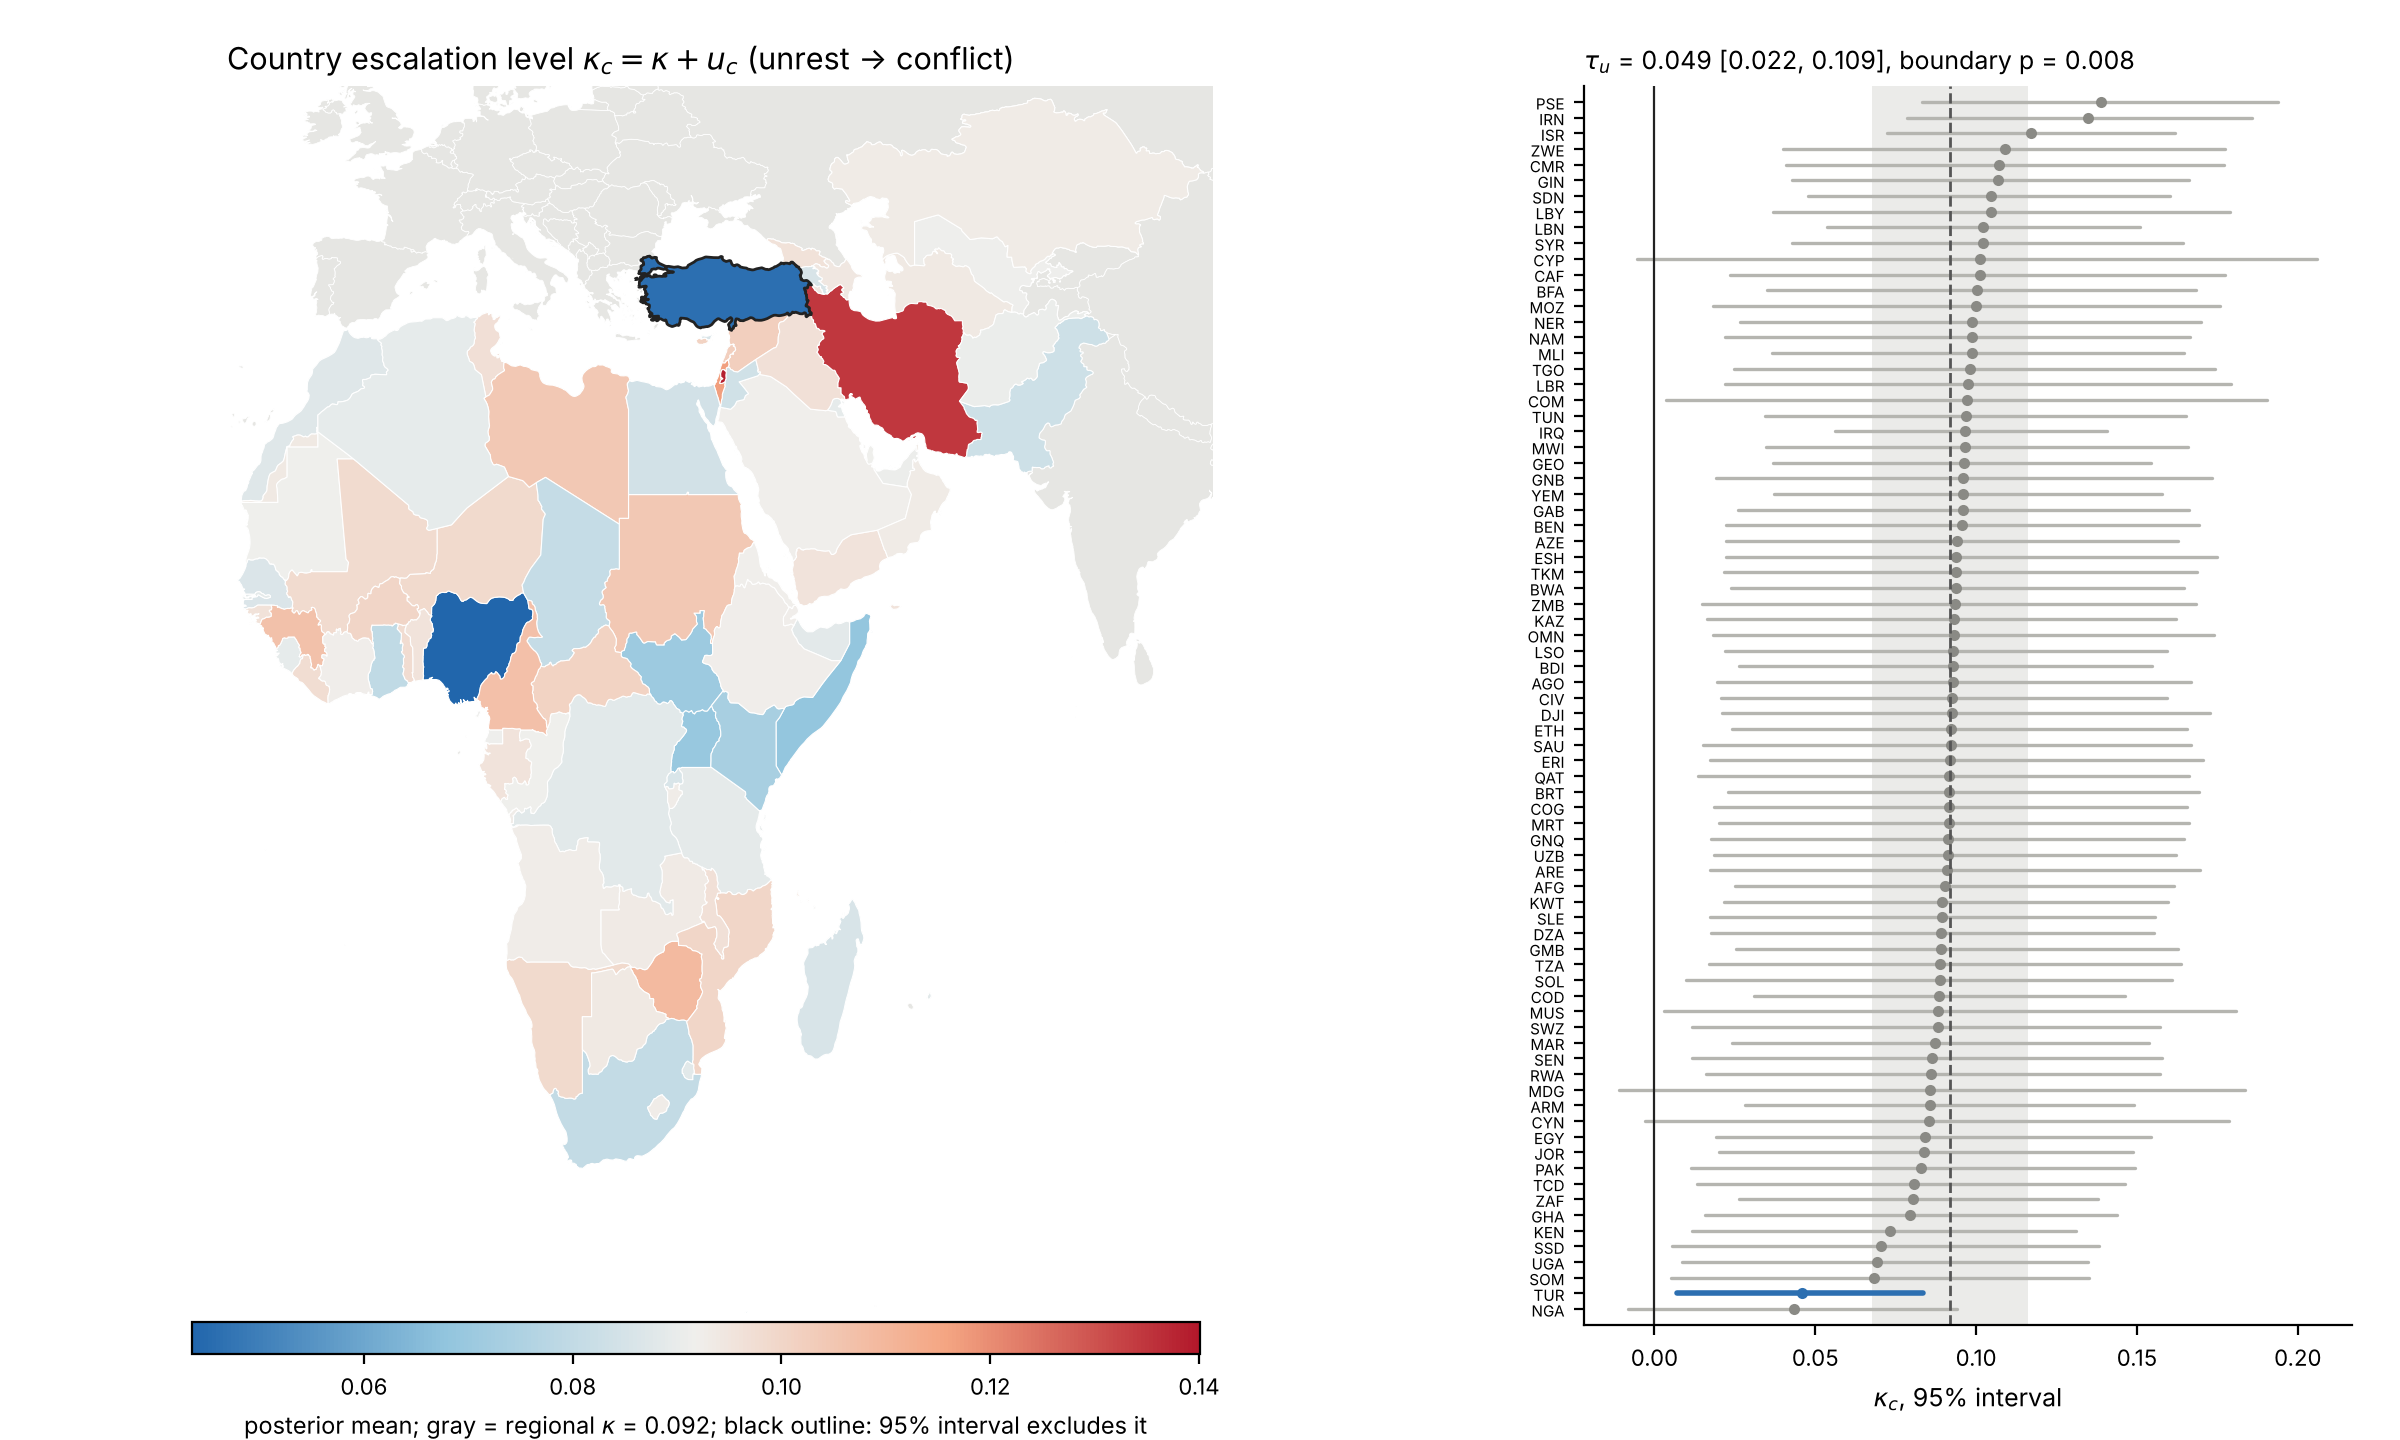
\includegraphics[width=\textwidth]{fig_country_kappa_ame_conflict.png}\end{center}

\textbf{Next}: one joint fit with $\bm\psi$ and $u_c$ (iid) for the final intervals; relaunch the three-outcome model.

\section*{Evidence so far (Africa and the Middle East; West Africa in brackets)}
{\footnotesize\setlength{\tabcolsep}{4pt}\begin{tabular}{@{}lll@{}}
\toprule
component & estimate, 95\% interval & reading \\
\midrule
$\delta_{\C}$ & 0.61 [0.59, 0.63] \; (0.45 [0.41, 0.48]) & supported \\
$\kappa_{\U\to\C}$, no shared cell effect & 0.094 [0.065, 0.123] \; (0.095 [0.032, 0.158]) & supported \\
$\kappa_{\U\to\C}$, with shared cell component & 0.057 [0.028, 0.086] \; (0.061 [$-$0.001, 0.123]) & modest \\
$\kappa_{\C\to\U}$, with shared cell component & 0.047 [0.020, 0.075] \; (0.076 [0.015, 0.137]) & modest \\
$\kappa_{\U\to\C}$, shared cell component, $\lambda = 0$ & 0.078 [0.049, 0.107] \; (0.092 [0.029, 0.154]) & inflated by 40--50\% \\
neighbours' unrest (dropped) & $-$0.011 [$-$0.021, $-$0.001] \; ($-$0.005 [$-$0.021, 0.011]) & about zero \\
lagged unrest, 13--26 weeks (dropped) & field diagnostic: corr. $-$0.04 \; ($-$0.08), placebo $\approx 0$ & no signal \\
$\lambda$ (shared episodes) & 0.35 [0.28, 0.42]; log-ML vs $\lambda = 0$: +60.7 \; (+19.8) & supported \\
shared cell component & loading 1.14 [1.05, 1.23], SD 1.46 [1.32, 1.61], range 44 [36, 53]\,km & supported; \\
 & (loading 1.68 [1.28, 2.08], SD 1.02 [0.85, 1.22], range 45 [31, 65]\,km) & implied $\rho_e \approx 0.89$ (0.92) \\
$\sigma_{e,\C}$ next to it & 0.16 [0.06, 0.45] \; (0.16 [0.03, 1.00]) & poorly identified: use $\rho_e$ \\
$\varphi_{\C}$ per block, range $\rho_{\C}$ & 0.89 [0.85, 0.91], 504 [455, 557]\,km \; (0.89 [0.84, 0.93], 426 [356, 510]\,km) & supported \\
$\sigma_{\U}$, $\varphi_{\U}$ (unrest only) & [0.40, 0.50], [0.54, 0.73] \; (0.55 [0.46, 0.65], 0.70 [0.55, 0.81]) & supported \\
$\sigma_{w,\U}$ (static unrest field) & 0.62 [0.48, 0.80] \; (0.50 [0.25, 0.99]) & away from zero: revisit drop \\
$\gamma(s)$, smooth & semi-synthetic (West Africa): see below & not detectable \\
$\lambda(s)$ & --- & not yet tested \\
\bottomrule
\end{tabular}}

\textbf{Reading of the new evidence.}
\begin{itemize}
\item \emph{Shared episodes} ($\lambda$). Setting $\lambda = 0$ lowers the log marginal likelihood by 60.7 (19.8 in West
Africa) and raises $\hat\kappa_{\U\to\C}$ from 0.057 to 0.078 (0.061 to 0.092) and $\hat\kappa_{\C\to\U}$ from 0.047 to
0.072 (0.076 to 0.110): without the channel, shared episodes are read as escalation. Channel 3 stays.
\item \emph{Shared places.} The shared static field has range 45\,km, below one cell, so it acts as a shared cell effect,
and it leaves $\sigma_{e,\C}$ unidentified (interval 0.03--1.00); the Hessian of the full model at its saved estimate is not
positive definite. It is replaced by the correlated cell effects $(e_{\C,s}, e_{\U,s})$, three parameters for the three
identifiable quantities; the saved fit implies $\rho_e \approx 0.92$.
\item \emph{Spatially varying escalation.} Outcomes regenerated from the fitted model on the West Africa design, with
$\gamma_{\U\to\C}$ a Mat\'ern field (10 replicates each). With $\gamma \equiv 0$, cell-level 95\% intervals almost never
exclude $\hat\kappa$ (mean 0.07\% of cells), but the posterior-mean spread of $\kappa(s)$ (q90$-$q10) averages 0.069 (up to
0.24, with sign reversals in up to half the cells). With $\sigma_\gamma = 0.061 = \hat\kappa$ (true spread 0.15) the fitted
spread averages 0.041, 0.1\% of cells are flagged, coverage is 0.94 and the correlation with the truth is 0.17. The null spread
exceeds the recovered planted spread: a smooth $\gamma(s)$ of the size of $\kappa$ is not detectable in one region. Spatial
differences in escalation are instead carried by the conditions $\bm\psi$ and the country levels $u_c$, read from
intervals, never from maps of posterior means.
\item \emph{Conditions, first test} (Task 44): superseded by Task 50 above.
\item \emph{Static unrest field.} With the shared cell component in the model, $\sigma_{w,\U}$ has an interval away from zero
in both regions (range 800--1000\,km, about the size of a country group). Its earlier drop rested on an older fit; under our
rule it should be kept, or kept as an uninterpreted control. To be decided.
\end{itemize}
\end{document}
